\chapter{Evaluation}

At first, the results of the methods on single robots must be investigated
in order to evaluate the performance of the final localization algorithm.
Depending on the accuracy of the individual direction results, the quality
of the team decision is limited.

Primary, whistle sounds were recorded in the laboratory of the HULKs.
If not emphasized particularly, the height of the sound source is 1.5\si{m}.
% signal start detection evaluation

First, the result of the direction detection on one robot
is examined profoundly with one measurement as an example.
There, we focus on the correctness and precision of the different methods.
To investigate the final localization of the team, measurements were
done with five robots on the field.
At the end, all measurements are used to assess the methods in a general matter.

In the following, the correlation function $R_{x_ax_b}$ of two signals
$x_a$ and $x_b$ as in \cref{chap:02_prerequisites} is shortened
to $R_{ab}$ for simplicity.

\section{Signal Start Detection}
\label{sec:04_signalStartDetection}

\todo[inline]{This section seems a bit misplaced. I feel like "Team Evaluation"
should be the last evaluation section. Is there a reason why you can't put this
before that?}

In previous chapters, the importance of the signal start was emphasized.
% Due to the fact that the direction detection methods is
% executed on smaller frames than the actual whistle detection.
% To demonstrate this for the phase method, the frame to examine is
% shifted with time \cref{subsec:04_frameNumber}.
Especially the result in \cref{subsec:03_phase} has shown that in fact, the
accuracy of the direction predictor decreases when evaluated on later samples
of the whistle signal.\todo{Maybe interpret this somewhere: give a reason
why shit makes sense (e.g. maybe because more reflections of the signal will
have reached the microphone)}
Also according to the outcome of \cref{subsec:04_psnr}, the \ac{GCC}
method performs best with frames near to the signal start. \todo[inline]{Get
rid of some cross-references and/or write more about what happened in these
chapters. (I don't remember what happened in 3.4 and 4.2.3 and jumping back and
forth is annoying.)}

% There are some reasons why other methods were tested to find the signal start.
In order to find a good solution for a highly reliable, accurate but
computationally tractable start detection, different approaches were
tested profoundly.
For high temporal\todo{I added "temporal" here because otherwise it seems unintuitive
that a less samples is better (because at the same time it might be harder to
predict from fewer samples as there is less information in the frame)} accuracy
either the number of samples in a frame have to be small\todo{Maybe rather say
that the frame as to be small? A low number of samples in a frame could also be
achieved by a smaller sampling rate, which would not help.} or the window must
be shifted with small steps which both implicit a large number of evaluations.
The existing whistle detection algorithm of the HULKs presented in
\cref{subsec:03_whistleDetection} is computationally intensive and has a low
accuracy for small frames\todo{Is "frames" actually the correct term (in
general)? Shouldn't it be "window"? I don't know what people use in signal
processing literature} as shown in \label{subsec:04_whistleDetection}.
Therefore, the goal is to identify a\todo{"looked" doesn't work this way. You are using this
quite a lot. Maybe grep the document for it and replace it.} simple algorithm for
the signal start detection. Ideally, this algorithm should be adaptable to
signals other than the whistle sounds.\todo{I would add a reference to the section
where you presented these algorithms. (this is only the evaluation, right?)}

Hereinafter, the performance of each method methods is evaluated by
analyzing the error between algorithmically determined start index
and manually labelled start index.
As a benchmark, the prediction accuracy is evaluated on 11 measurements on all
robots\todo{how many robots?} \todo{this sentence is missing some
words}\cref{subsec:04_labMeasurements}.
By the frame size of the \ac{FFT} being set to 256 samples for the
correlation methods, a start index error of at most 256 samples is
desired.
Therefore, a start index detection result is regarded as failure for errors
larger than 256 for the following sections.
Two metrics are specified to express the degree of failure.
The former counts the number of large errors for each channel.
In this case, 220 sample data for 11 measurements on five robots with
four channels each exist.\todo{I don't understand this sentence.}
The second metric reports the number of measurements for which any of the
channels failed. For this case, 55 measurements are given.\todo{Again, what is
this sentence saying? I thought we had 11 measurements? Or is it 11
measurements * 5 robots? Maybe simply write 55 in the first place (rather than
11)}.
% -----------------------------------------------------------------------------------------------------

\subsection{Whistle Detection}
\label{subsec:04_whistleDetection}

\todo[inline]{It is not immediately clear that with "whistle detection" you refer
to the "whistle detection of the HULKs", e.g. your "baseline"}
First, the accuracy of the whistle detection in regard of the start index
is evaluated.
Here, the start index is defined as the first index where the whistle detection
found a whistle.
With a frame size of 1024, the whistle detection algorithm fails in every of the
55 measurements with at least one channel if only an error of at most 256 samples
is permitted.
However, every error is in the range of 1024 samples which proves that the
approximate start of the whistle sound is detected correctly.
With a smaller frame size of 256, the temporal accuracy is improved but
introduces false positive detections.\todo{do you have numerical results here?}
With the results, one can say that the whistle detection is not sufficient
for the start detection or is at least not reliable as stand-alone solution.
Furthermore, this approach is limited to sounds in fixed and known frequency range.
%  failure rate of
% 9\si{\percent} in regard to every channel.
% In this work microphone data were saved as soon as the whistle detection module
% found a whistle sound in the audio samples.
% Due to this implementation, the algorithm does never fail to detect the whistle
% Standing alone, the error is always in the range of \si{\pm1024} samples due to the
% set frame size of 1024 samples.
% With a smaller frame size of 256, the accuracy gets better with an error of
% 9\si{\percent} in regard to the 220 sample data but has an error rate of
% 25,5\si{\percent} for the measurements.

% looking at the next 300
% values and with a step size of 50 the result is 15\si{\percent} and 36\si{\percent}
% and with step size 1, it is 13\si{\percent} and 33\si{\percent}.
% This is computationally very costly and the reward is small.

\subsection{ZCR}
\label{subsec:04_zcr}

For the evaluation of the \ac{ZCR},
the frame size is set to 256 samples and number of noise and signal frames
are set to 10 frames.
In 7\si{\percent} of the 220 channel sample data\todo{"sample data" sounds like
it is not a term. Maybe only "samples"?}, the method fails with a significant
error larger than 256 samples.\todo{I don't thing you have to repeat the 256
sample criterion every time. You defined what is considered a failure earlier.
Just say "failed".} In most cases, the method provides accurate results with
small error. Taking all measurements of robot 26 as example, the \ac{RMSE}
amounts 54.23 samples.\todo{Again, where is the data for this? Tables, figures?}

However, there are cases where the algorithm fails. Looking at those cases it
could be identified that the errors occur often due to incorrect assumptions
that the signal is present at the end of the buffered samples.
Some measurements prove that this is not always the case as shown in
\cref{fig:04_zcrFail}.
Here, the data of the front right channel of robot 21 with the whistle source
at position 5 in \cref{subsec:04_labMeasurements}
illustrates how the signal ended around 35000 samples already. \todo{Neither
the robot number, nor the position or the channel are relevant here I think.}
If the start index is determined at the point where the \ac{ZCR}
falls below the threshold searching backwards as stated in \cref{sec:02_signalStartDetection},
the detection fails.

In most cases, only one out of four channels produces a erroneous
result.\todo{Why? Doesn't the signal end early on all channels?}
Because the final start index on one robot is set equal for all channel,
the failure can be compensated with a simple voting procedure.
% -------------------------------------------------------------
\begin{figure}[ht]
	\centering
	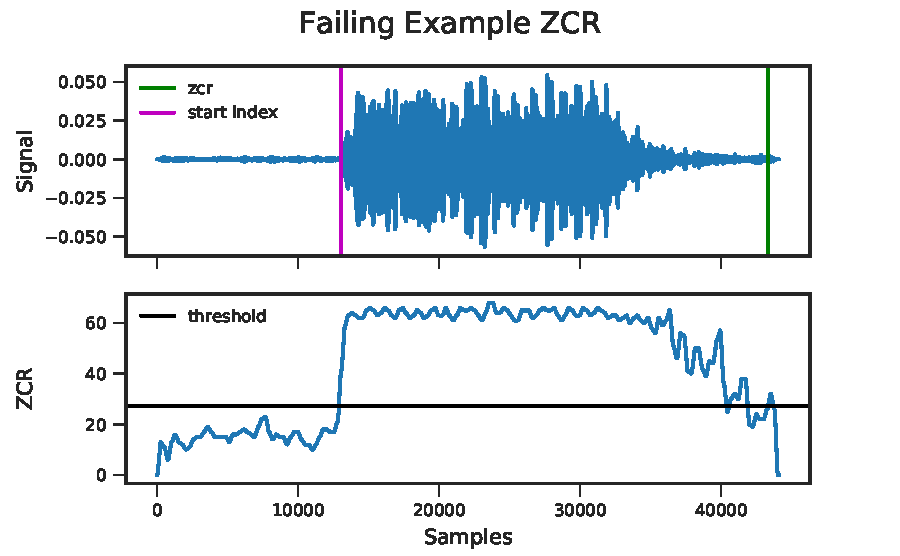
\includegraphics[]{figures/evaluation/zcr_fail}
	\caption{Channel 3 data from measurement 5 of \cref{subsec:04_labMeasurements}
		for robot number 21. A failing example for the start detection by \ac{ZCR}
		is shown.}
	\label{fig:04_zcrFail}
\end{figure}
% -------------------------------------------------------------
If the start index is determined at the point where the \ac{ZCR}
falls below the threshold searching backwards as stated in \cref{sec:02_signalStartDetection},
the detection fails.

In most cases, only one channel of four output a erroneous result.
Because the final start index on one robot is set equal for all channel,
the failure can be compensated with a smart voting procedure.

Another option exists by changing the process of finding the
threshold excess onwards.\todo{I don't understand what this is saying.}
In this case, the threshold is scaled with a factor of 1.25.
Results by this were poorer than the initially implemented manner
with a failure rate of 15\si{\percent}.\todo{Did you ever report the previous failure rate?}
By adding the constraint that multiple samples must exceed the
threshold successively, result can be slightly improved for the cost of higher
computational effort.

It should be noted that the poor performance of the \ac{ZCR} method with signal that
was cleaned with spectral subtraction previously. This surprising outcome is
convenient for the overall task, because the start index result can be embed
into the spectral subtraction, providing information for separating the noise
and signal part.\todo{I don't get what this paragraph is saying?}

\subsection{Entropy}
\label{subsec:04_entropy}

As discussed in \cref{subsec:02_Entropy} the entropy quantifies the amount
of chaos in a signal frame.\todo{Is this correct? Chaos is deterministic and not
the same as randomness}
Especially for signals to localize with unknown characteristics,
this method can be useful because no a-priori knowledge is needed.\todo{You should
probably say that the only prior knowledge must be, that the signal to detect
has lower entropy than the background noise.}
For all measurements this method yielded poorer results than the \ac{ZCR} method
with a failure rate of around 20\si{\percent}.
Best results are achieved with a frame size of 512 samples and a step size of 800
samples.
% \change[]{Explain what steps are? Maybe in implementation?}
However, for records with fading whistle the entropy method
generates more reliable results than the \ac{ZCR} method.\todo{What do you mean
by "fading whiste"? Whistles that don't have a distinct/abrupt start?}
Taking the same measurement as an example for which failure of the \ac{ZCR} method
was discussed earlier, \cref{fig:04_entropyGood} shows how the algorithm
detects the signal start correctly even though the whistle sound ended at
around 35000 samples. In this measurement, the start index errors of all four
channels were smaller than 40 samples.
% -------------------------------------------------------------
\begin{figure}[ht]
	\centering
	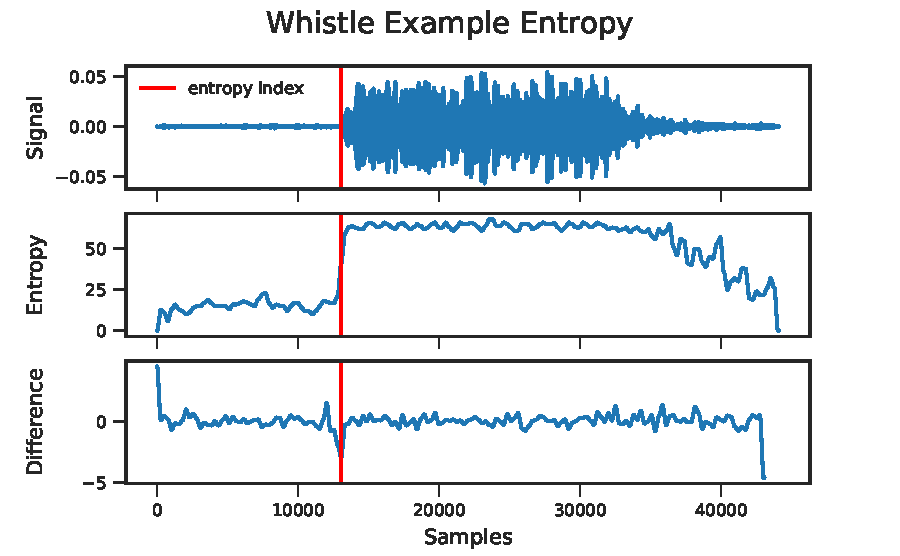
\includegraphics[]{figures/evaluation/entropy_good}
	\caption{Exemplary result of start index detection by entropy where
			the \ac{ZCR} method failed due to fading whistle
			at the data.}
	\label{fig:04_entropyGood}
\end{figure}
% -------------------------------------------------------------

% But as the entropy should be larger for noisy environment
% performance in other surrounding of measurement at \ac{RoboCup} is looked at.
% Entropy would be best for undefined signal -> distinguish between
% signal and noise without information

\section{\acl{WSDE}}
\label{sec:04_tdoaSingle}

Before evaluating the performance of the different methods as a whole,
% For comparability of the results,
one exemplary measurement is utilized
to present and analyse the \ac{TDOA} methods in detail first.
In this recording, the sound source is placed at the right front
of the robot with 4.5\si{m} distance.
Hereinafter, this measurement will be referenced to as \textit{demonstration-dataset}.
This corresponds to an an angle of -33.7\si{\degree} in robot coordinates.
To get an idea about the examined data, according whistle signal samples around the
start are plotted in \cref{fig:04_tdoaSignal} for all channels.
% -------------------------------------------------------------
\begin{figure}[ht]
	\centering
		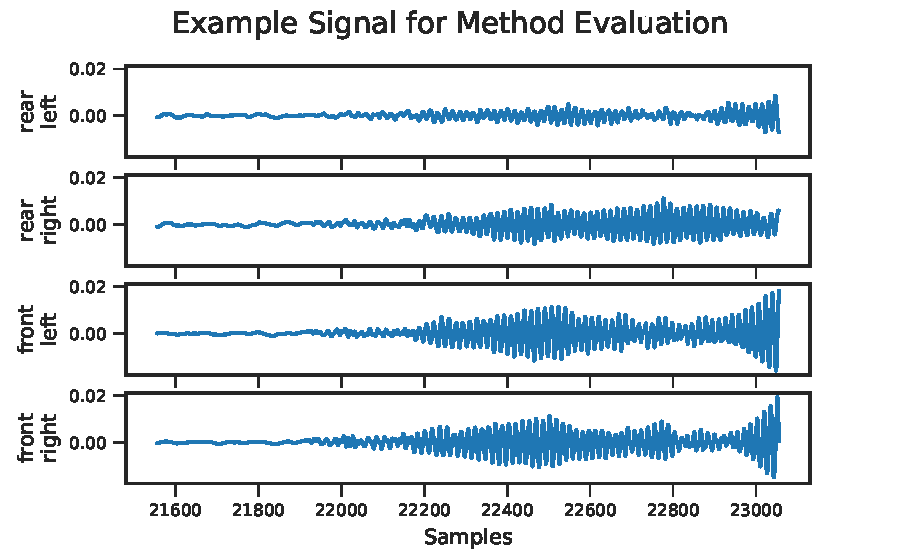
\includegraphics[]{figures/evaluation/cc_frontRight_1_signal}
	\caption{Signal start section of a whistle sound recorded from front right.}
	\label{fig:04_tdoaSignal}
\end{figure}
% -------------------------------------------------------------

As the next sections focus on the performance of the \ac{TDOA} methods,
the start index is set manually.

For the sake of conciseness, throughout the following sections the correlation
function $R_{x_ax_b}$ of two signals $x_a$ and $x_b$  (\cf
\cref{chap:02_prerequisites}) is denoted as $R_{ab}$.


\subsection{Cross Correlation}
\label{subsec:04_ccSingle}
% -------------------------------------------------------------

The \ac{CC} is a widespread technique to obtain the time delay
between two series of samples.
To discuss the result of the \ac{CC}, the belonging correlation functions
of the demonstration-dataset are plotted in \cref{fig:04_cc}.
The selection process and implementation correspond to the explanations
in \cref{subsubsec:03_cc}.
For $R_{32}$ and $R_{13}$ a peak is clearly visible.
However, for the other \ac{CC} the problem of a weak peak
arises what was mentioned as downside of the \ac{CC} in \cref{sec:02_cc}.
% -------------------------------------------------------------
\begin{figure}[ht]
	\centering
		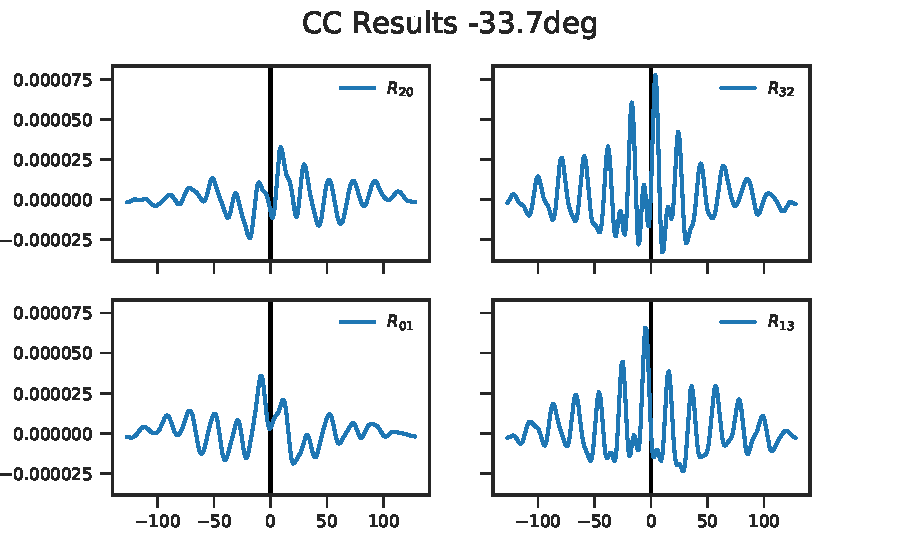
\includegraphics[]{figures/evaluation/cc_frontRight_1}
	\caption{Cross correlation results of signal from front right (-33.7\si{\degree}).}
	\label{fig:04_cc}
\end{figure}
% -------------------------------------------------------------
\btline{ht}{1.2}
\btab{|c|c|c|c|c|}
\hline
Base Channel & Next Channel & Delay & Candidate (-) & Candidate (+)\\
\hline
0 & 1 & -8.25 & -144.9 & -35.1\\
\hline
1 & 3 & -4.59 & -17.4 & 78.6\\
\hline
2 & 0 & 9.16 & -30.6 & -30.6\\
\hline
3 & 2 & 3.94 & -150.2 & -29.8\\
\hline
\etab
\et{Cross correlation delay results of signal from front right}{04_cc}
% -------------------------------------------------------------

According to the delays in \cref{tab:04_cc}, two source direction candidates arise
for each channel pair.
By the implementation in \cref{subsec:03_directionCandidates}, the combination of
all options with the smallest error is selected as \ac{WSDE}.
Hence, the algorithm outputs -26.9\si{\degree} what produces an error of 6.8\si{\degree}.
The delay between channel 2 and 0 is larger than the maximum delay of 6.85 samples
and therefore cut to the maximum sample delay.
Besides these, the \ac{TDOA} between the channel pairs produce one appropriate
direction candidate which correctly points to the sound source.
% -------------------------------------------------------------

\subsection{Generalized Cross Correlation}
\label{subsec:04_gccSingle}
% -------------------------------------------------------------
\Cref{fig:04_gcc} presents the \ac{GCC} result by the \ac{GCC-PHAT} method of
the demonstration-dataset equal to \cref{subsec:04_ccSingle}.
The subsample delays for each channel pair and their resulting direction candidates
are listed in \cref{tab:04_gcc}.
From this, a final direction of -30.0\si{\degree} is determined
resulting in an error of 3.69\si{\degree}.
It is apparent that the peaks of the \ac{GCC} are better to detect than the peaks of the
\ac{CC}.
% -------------------------------------------------------------
\begin{figure}[ht]
	\centering
		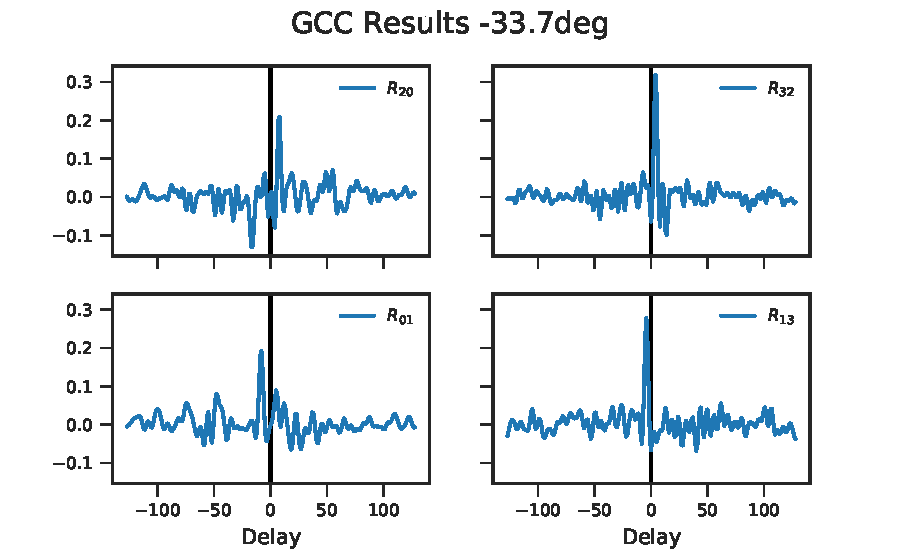
\includegraphics[]{figures/evaluation/gcc_frontRight}
	\caption{Generalized cross correlation results of signal from front right.}
	\label{fig:04_gcc}
\end{figure}
% -------------------------------------------------------------
\btline{ht}{1.2}
\btab{|c|c|c|c|c|}
\hline
Base Channel & Next Channel & Delay & Candidate (-) & Candidate (+)\\
\hline
0 & 1 & -8.28 & -144.7 & -35.3\\
\hline
1 & 3 & -4.09 & -22.8 & 84.0\\
\hline
2 & 0 & 7.60 & -30.6 & -30.6\\
\hline
3 & 2 & 4.13 & -148.7 & -31.3\\
\hline
\etab
\et{Generalized cross correlation delay results of signal from front right}{04_gcc}
% -------------------------------------------------------------
\subsection{Phase Difference}
\label{subsec:04_phaseSingle}

For detecting the source direction with phase difference, a smaller frame
size of 64 samples is defined.
In \cref{subsubsec:03_phase} two variants of this method were introduced that use
different strategies to identify a reference frequency. The first version uses
a static reference frequency that is fixed a-priori by the user. The second version
dynamically estimates a dominant frequency across all four channels. Hereafter,
the performance of both variants is discussed.


\subsubsection*{Static Reference Frequency}

In \cref{subsubsec:03_phase} two different ways to set a reference frequency $f_c$
for the phase difference method were introduced.
First, a suitable value for the reference frequency is specified by
examining the influence of the chosen value.
Therefore, \ac{WSDE} results with the phase difference method are evaluated by setting
different values for the reference frequency within whistle range.
For this purpose we consider all of eleven measurements of the the laboratory-dataset
recorded with robot no. 26 at the center point.

According to \cref{subsubsec:03_phase}, the most feasible frequency is defined as
2775.08\si{\hertz} by the distance between the channels
and the whistle spectrum ranges between 2\si{\kilo\hertz}
and 4\si{\kilo\hertz}.

As shown in \cref{fig:04_diffFc} shows, the \ac{RMSE} is high for
frequencies smaller than 2600\si{\hertz}.
With a frequency of 2024.12\si{\hertz}, error is largest.
% The result complies with the information in \cref{fig:03_maxFreq} showing that
% frequencies higher than 2500\si{\hertz} are dominant in whistle signals.
With this outcome, the fixed frequency is set to 2670.1\si{\hertz}
for further usage of the direction detection by phase method.
Limitation exists due to the ambiguity of the signal which is
content of \cref{subsubsec:03_phase}.
% -------------------------------------------------------------
\begin{figure}[ht]
	\centering
		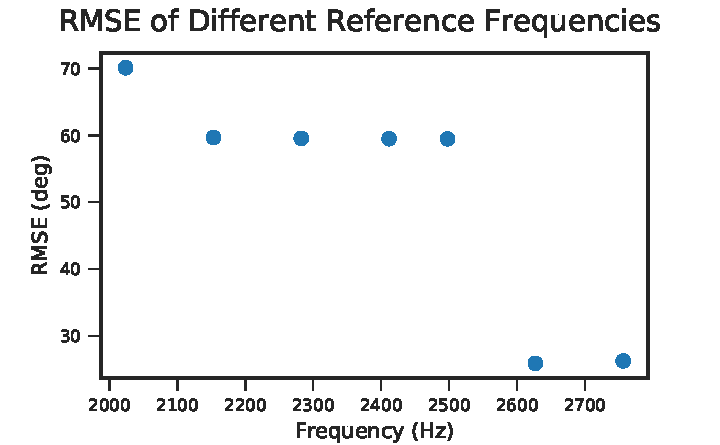
\includegraphics[]{figures/evaluation/phase_fc_rmse}
	\caption{Result of all measurements done with robot 26 to compare different
	fixed frequency values in whistle range.}
	\label{fig:04_diffFc}
\end{figure}
% -------------------------------------------------------------

On the basis of the results, the reference frequency was set to a minimum
of 2600\si{\hertz} for evaluation of the demonstration-dataset.
Hence, the reference frequency is 2627.1\si{\hertz} in the case of a \ac{FFT} length
of 256 samples.
Applying the phase difference method with this reference frequency, the final
direction estimate computed from the candidates listed in
\cref{tab:04_fixedFreqResult} is -29.6\si{\degree} which results in an error of
4.1\si{\degree}.
% -------------------------------------------------------------
\btline{ht}{1.2}
\btab{|c|c|c|c|c|}
\hline
Base Channel & Next Channel & Phase Difference & Candidate (-) & Candidate (+)\\
& & [\si{\deg}] & [\si{\deg}] & [\si{\deg}] \\
\hline
1 & 3 & -79.1 & -26.8 & 88.0\\
\hline
2 & 0 & 167.7 & -30.6 & -30.6\\
\hline
3 & 2 & 88.5 & -148.7 & -31.3\\
\hline
\etab
\et{Resulting candidates of phase difference method with fixed frequency
	2670.1Hz of example measurement from front right
	(-33.7\si{\degree})}{04_fixedFreqResult}
% -------------------------------------------------------------

\subsubsection*{Dynamic Reference Frequency Selection}

Another option is to have a nonspecific reference frequency that
is computed dynamically without a-priori knowledge.
As stated in the implementation chapter, frames are chosen where the frequencies
of the maximum amplitudes coincides for all channels.
For the running example discussed here, this corresponds to a frequency of 2756.25\si{\hertz}.

For comprehensibility, the determined frequency information visualized by
wave signals with the detected phases and amplitudes
in the lower subplot of \cref{fig:04_phaseSingle}.
In the upper plot of \cref{fig:04_phaseSingle} one sees the originally received microphone
data before applying a Hann window and transforming it into frequency domain by
\ac{FFT}. The resulting phases and amplitudes are listed in
\cref{tab:04_phaseSingle}.
% -------------------------------------------------------------
\begin{figure}[H]
	\centering
		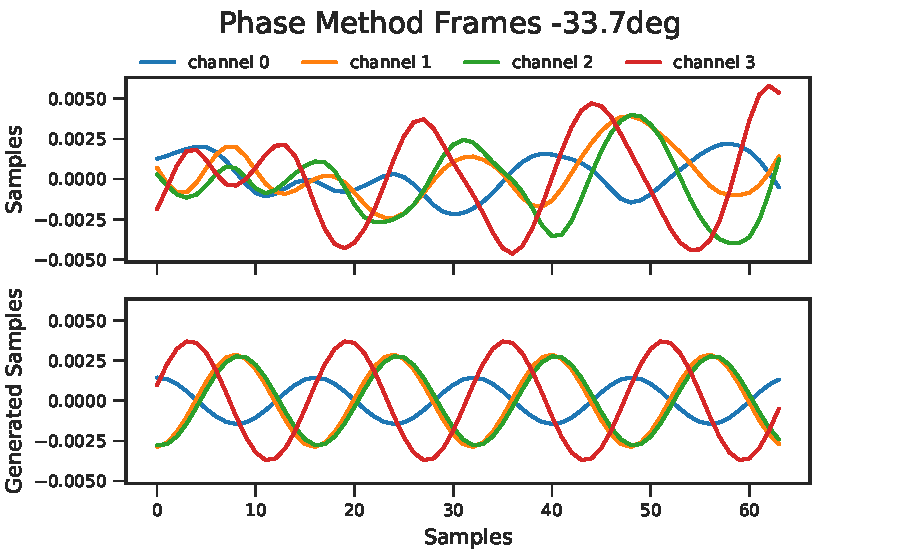
\includegraphics[]{figures/evaluation/phase_cos}
	\caption{Frames used for the direction detection by phase method.}
	\label{fig:04_phaseSingle}
\end{figure}
% -------------------------------------------------------------
\Cref{tab:03_maxFrequencies} pointed out that the most feasible frequency
of the rear channels 0 and 1 is not in whistle spectrum
due to the larger physical distance between the microphones.
Thus, the phase difference information is neglected because of the ambiguity of
the temporal sequence between the signals.
Following the procedure discussed in \cref{subsubsec:03_phase},
the resulting phase difference estimate
is -29.2\si{\degree} by combining the candidate direction -17.6\si{\degree},
-30.6\si{\degree} and -39.3\si{\degree} from channels 1, 2 and 3 according to
\cref{tab:04_phaseDiffSingle}.
% -------------------------------------------------------------
\btline{ht}{1.2}
\btab{|c|c|c|}
\hline
Channel & Phase [\si{\deg}] & Amplitude\\
\hline
0 & -1.55 & 0.00144\\
\hline
1 & -177.7 & 0.00287\\
\hline
2 & 173.4 & 0.00279\\
\hline
3 & -75.0 & 0.00372\\
\hline
\etab
\et{Phase and amplitude of frame signals with $f_c$ = 2756.25Hz}{04_phaseSingle}
% -------------------------------------------------------------
\btline{ht}{1.2}
\btab{|c|c|c|c|c|}
\hline
Base Channel & Next Channel & Phase Difference & Candidate (-) & Candidate (+)\\
& & [\si{\deg}] & [\si{\deg}] & [\si{\deg}] \\
\hline
1 & 3 & -102.7 & -17.6 & 78.8\\
\hline
2 & 0 & 173.4 & -30.6 & -30.6\\
\hline
3 & 2 & 113.1 & -140.7 & -39.3\\
\hline
\etab
\et{Phase differences and resulting direction candidates of demonstration-dataset
with dynamically determined reference frequency}
{04_phaseDiffSingle}
% -------------------------------------------------------------

\subsubsection*{Impact of Selected Frame}
\label{subsubsec:04_frameNumber}

Not only does the frequency play a major role for the phase method,
but also the samples chosen for analysis.
Again it is referred to the eleven measurements of the laboratory-dataset
recorded on the robot at the center point (no. 26).
To evaluate if and how the result changes over time, the selection window
is shifted by half the frame size from -5 shift steps to 20.
Recapitulating the implementation details for the static reference frequency case
in \cref{subsec:04_phaseSingle},
the first frame after the start index is chosen in which the whistle detection would
count a whistle signal.
This frame is represented by zero shift.

% [ 62.32629763  59.19634105  66.78950798  54.53898736  30.80692207
%   25.91537359  56.55427899  65.27548831  66.3898905   75.48670644
%   97.33965933  96.6373387  100.22012166 104.20160752  59.55737843
%   58.22148221  48.51237213  51.93254436  49.08273252  62.64453085
%   56.49506079  57.03430393  67.46509351  73.21671739  43.69704948]
In \cref{fig:04_phaseOverTime}, the resulting errors per shift
for all measurements are plotted, presenting the influence of the
selected frame around the signal start.
The reference frequency was set to 2627.1\si{\hertz} due to the
outcome that frequencies larger than 2600\si{\hertz} achieve best results.
The graph presents that frames nearest to the signal start reach best results
with an \ac{RMSE} of 25.9\si{\degree}.
These results show that the frame position has a significant influence on the prediction
accuracy of the direction detection.
Therefore, an accurate signal start detection is crucial for the preciseness of the \ac{SSL}
by phase difference.
% -------------------------------------------------------------
\begin{figure}[ht]
	\centering
		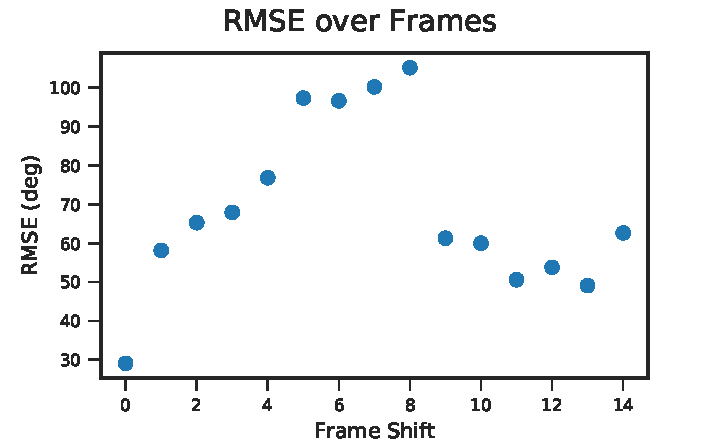
\includegraphics[]{figures/evaluation/phase_over_time}
	\caption{\ac{WSDE} result errors while shifting the frame over the
	samples of the laboratory-dataset on robot no 26.}
	\label{fig:04_phaseOverTime}
\end{figure}
% -------------------------------------------------------------

\subsubsection*{Phase Method Conclusion}
\label{subsubsec:04_phaseMethodConclusion}

Different options were investigated relating to the phase difference method
in the last subsections.
One finding is that reference frequency values should be chosen larger than
2.6\si{\kilo\hertz} for best results.
Another is that samples at the beginning of the signal are most suitable
for this method.
An advantage of the dynamically selected reference frequency is the reduction of
one parameter.
It requires more effort to implement and considering edge cases but
does not depend on the whistle detection.
Both approaches are valid for this work and result in a similar reference
frequency due to the limitations listed in \cref{subsubsec:03_phase}.

\subsection{\ac{TDOA} Method Comparison}
\label{subsec:04_singleRobotAngleError}

As the different \ac{TDOA} methods were discussed profoundly in the last
sections, all measurements of the laboratory-dataset are considered here
to make a generalized statement about the performance.
The \acp{WSDE} resulting from here are the inputs of the multi-agent
localization filter.
\Cref{fig:04_compareRmse} presents the \ac{RMSE} considering the
direction results of all five robots for each measurement in
\cref{subsec:04_labMeasurements}.
Additionally, the estimated standard deviation of each measurement
provides insight into the validity of the single robot results.
As one can see, the standard deviation of the relative angle of the \ac{GCC}
method is significantly smaller as compared to the phase method for most
measurements.
How this influences the reliability of the sound localization is
subject of discussion in \cref{sec:05_methodComparison}.
% -------------------------------------------------------------
\begin{figure}[h]
	\centering
		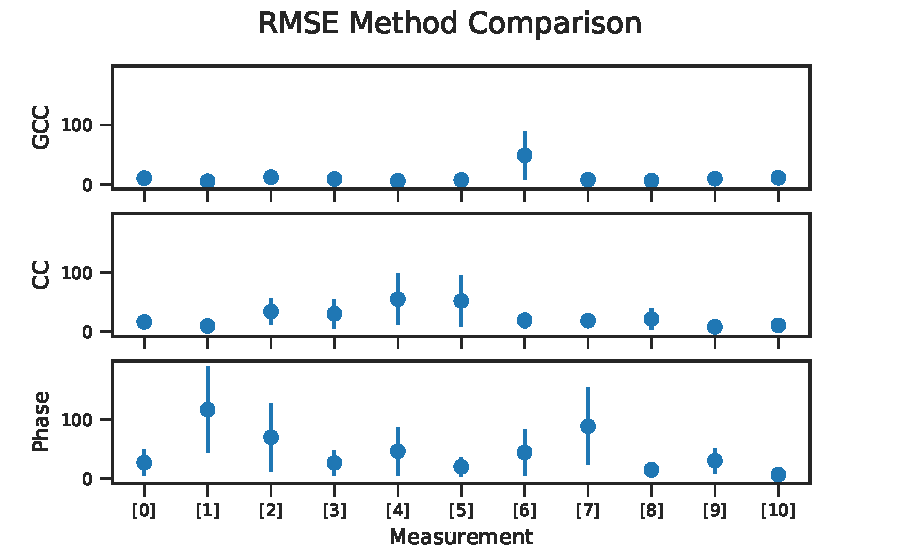
\includegraphics[]{figures/evaluation/compare_rmse}
	\caption{Angular RMSE and standard error of robot results per
	measurement of \cref{subsec:04_labMeasurements}.}
    \label{fig:04_compareRmse}
\end{figure}
% -------------------------------------------------------------

\subsection{Conclusion}
\label{subsec:04_tdoaConclusion}

The results in \Cref{subsec:04_singleRobotAngleError} show
that the \ac{GCC-PHAT} algorithm performs best according to the
laboratory-measurements.
Not only the errors are smallest, but also the low standard deviation
displays that the robots agree on the \ac{WSDE} and little outliers exist.
Also in regard to the multi-agent Bayesian updating filter, unified
results of the stand-alone robots are beneficial.
Another advantage of the \ac{GCC-PHAT} method is the presence of
a indication regarding the certainty of the measurement.
Interpreting the \ac{PSNR} as such, it can be used to detect outliers
or consider results with small \ac{PSNR} less.
\section{Distance Measurements}
\label{sec:04_distance}

To examine this, measurements from the front and back of the robot were
collected and evaluated.
\section{Team Evaluation}
\label{sec:04_teamEvaluation}

\change[]{correct}
First, the start indexes were set manually to provide a decoupled result.
The size of the field used in this work is smaller than the regular \ac{SPL}
field. It's length is 7.5\si{m} and it's width is 5\si{m}.
It is looked at the result of one exemplary measurement where the behavior
of the team filter is of prime importance.

\subsection{Measurement Setup}
\label{subsec:04_labMeasurements}
In order to evaluate the localization methods, 11 measurement were
taken. \Cref{fig:04_setup} illustrates the positions of the Nao robots
and the positions of the whistle sound source.
According to these. the x and y values of the sources and robots are
listed in \cref{tab:04_robots} and \cref{tab:04_sources}.
The angle $\theta$ of the robots are relative to the x-axis and
corresponds to the definition in \cref{subsec:03_coordinates}.
In the following sections, the signal data from these measurements
will be used mainly.
% -------------------------------------------------------------
\btline{ht}{1.2}
\btab{|c|c|c|c|}
\hline
Nao & x [\si{m}] & y [\si{m}] & $\theta$ [\si{deg}]\\
\hline
21 & 3,75 & 2,5 & -40,2\\
\hline
24 & 3,75 & -2,5 & 90\\
\hline
26 & 0 & 0 & 0\\
\hline
27 & -3,75 & -2,5 & 66,06\\
\hline
28 & -2,45 & 0 & 0\\
\hline
\etab
\et{Positions of the robots for evaluation measurement}{04_robots}
% -------------------------------------------------------------
\btline{ht}{1.2}
\btab{|c|c|c|}
\hline
Number & x [\si{m}] & y [\si{m}]\\
\hline
[0] & 3,75 & 2,5\\
\hline
[1] & 3,75 & -2,5\\
\hline
[2] & -3,75 & -2,5\\
\hline
[3,9] & -3,75 & 2,5\\
\hline
[4] & -2,45 & 0\\
\hline
[5] & 2,45 & 0\\
\hline
[6,10] & 0 & 0\\
\hline
[7] & 0 & -2.5\\
\hline
[8] & -6.05 & 0\\
\hline
\etab
\et{Positions of the whistle sound sources for evaluation measurement}{04_sources}
% -------------------------------------------------------------
\begin{figure}[ht]
	\centering
		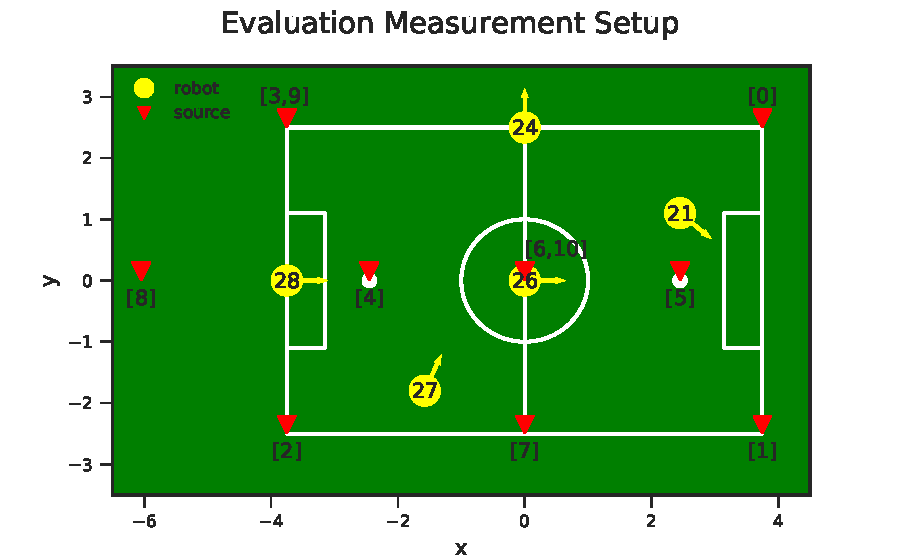
\includegraphics[]{figures/evaluation/setup}
	\caption{Setup of robots and sound source positions for the evaluation measurement.}
    \label{fig:04_setup}
\end{figure}
% -------------------------------------------------------------

\subsection{SNR}
\label{subsec:04_snr}

For the team filter, it the validity a robot result is useful information.
Depending on the uncertainty, the covariance of the incoming result can be adjusted.
Thus, one intuitive hypothesis is assuming the existence of a relation between the
received signal strength and distance to the source.
Taking the measurements of \ref{subsec:04_labMeasurements}, this hypothesis is
investigated by looking at the distance between one robot and the sound source.
According to this distance, it is looked at the \ac{SNR} of one measurement on
one robot proportional to all robots' \acp{SNR} of this measurement.
The \ac{SNR} on a single robot consists of the mean over all microphones' \acp{SNR}.
We can see in \cref{fig:04_snrDistance} that there is no straightforward
link between both values.
Also only taking a frame of size 256 samples into consideration
does not change the result.
% -------------------------------------------------------------
\begin{figure}[ht]
	\centering
		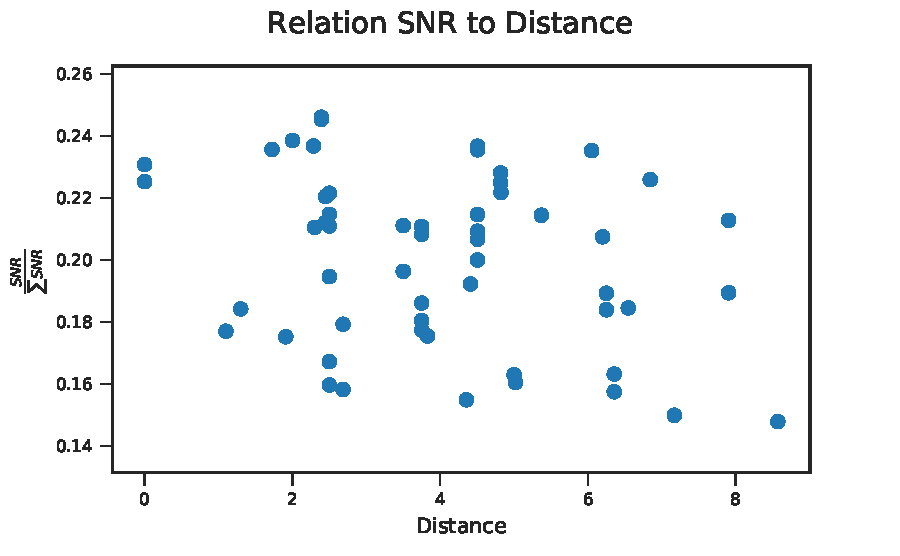
\includegraphics[]{figures/evaluation/snr_scatter}
	\caption{Visualization of relation between SNR and distance.}
    \label{fig:04_snrDistance}
\end{figure}
% -------------------------------------------------------------

Due to the unexpected result, further analysis on the \ac{SNR} values
on individual robots are done.
Therefore, a sine signal with fixed distance to the robot
was recorded from different angles with constant volume.
The main purpose of this measurement is to ensure that the lone channels
are not biased somehow.
Resulting from 14 measurements of a 3\si{\kilo\hertz} sine signal
with are distance of 0.73\si{m}, no tendency could be detected.
Further evaluation is done by determining the channel with the maximum
\ac{SNR} of one measurement. At 85,71\si{\percent} of the cases,
result coincided with the expected channel.
From this, we can say that the general recordings of the microphones
are neither biased nor falsified.

The same investigation is done with the real whistle recordings of the
measurement in \ref{subsec:04_labMeasurements}.
With these measurements only 54,55\si{\percent} of the maximum \acp{SNR}
match with the expected channels.
Consequentially, we must assume that the environmental circumstances
like multi-path propagation and reflection have large influence
on the signal magnitude.

\subsection{PSNR}
\label{subsec:04_psnr}

As referred in \cref{sec:02_gcc}, one characteristic of the \ac{GCC-PHAT}
algorithm is the sharp peak.
In conclusion, one can assume that if no sharp peak can be detected the
delay result of the \ac{GCC} has less informative value.
The validity of this statement is tested by comparing the \ac{PSNR} value
to the error of the direction angle resulting from the \ac{GCC-PHAT} delay.
Two cases of errors are taken into consideration.
In both, the \ac{PSNR} is recorded as high if it exceeds 17,5 whereat the
value ranges from 10,1 to 28,8.

Firstly, each channel pair on one robot is looked at by determining the
smaller error between the actual angle and one of both direction candidates.
If the \ac{PSNR} of the \ac{GCC} is greater than the threshold of 17,5,
the \ac{RMSE} of its result is grouped to the errors with high \ac{PSNR}.
Elsewise it pertains to the errors with low \ac{PSNR}.
This valuation is done with the measurements of \cref{subsec:04_labMeasurements}
and manually set start indexes.
Having 76 correlations assessed with low \ac{PSNR}, the \ac{RMSE} of these
is 35,77\si{\degree}.
Compared to this, the \ac{RMSE} of the remaining 144 measurements
is 15,86\si{\degree}.

To see the impact on a complete robot result, the same is done
with the final errors on single robots.
Here, the \ac{RMSE} of the lower \ac{PSNR} case results in 25,36\si{\degree}
whereat the error of the other case is 14,41\si{\degree}.

From this, one can identify the \ac{PSNR} as valid additional information
for the covariance of a \ac{GCC-PHAT} delay result that enriches the
outcome of a robot direction ray that proceeds into the team filter.